\documentclass[11pt,a4paper]{article}
\usepackage[utf8]{inputenc}
\usepackage[T1]{fontenc}
\usepackage[margin=2.5cm]{geometry}
\usepackage{array}
\usepackage{booktabs}
\usepackage{longtable}
\usepackage{enumitem}
\usepackage{tikz}
\usepackage[hidelinks]{hyperref}
\usepackage{xurl}
\sloppy

\title{Voluntary Saccades and Visual Stability: Spatiotopic vs Retinotopic Accounts}
\author{Francesco Mannella}
\date{October 4, 2026}

\begin{document}
\maketitle

\section{The problem}

Voluntary saccades, about 3 to 4 per second, shift the retinal image of the whole scene each time, yet the world looks stable; two families of explanation compete over where and how the brain compensates.

Each saccade (typically 200 to 300 ms apart) moves every object to a new retinal location, and the early visual system is retinotopic (\href{https://www.pnas.org/doi/10.1073/pnas.1812210116}{Fabius et al., 2019}). Perception, by contrast, is largely world-centred (\href{https://www.sciencedirect.com/science/article/pii/S1053811916306899}{Fairhall et al., 2017}). Two lines of explanation structure the field:

\begin{itemize}[itemsep=2pt,topsep=2pt]
\item \textbf{Spatiotopic (world- or head-centred) line.} The brain builds explicit maps in external coordinates by combining retinal position with eye-position signals (gain fields), and perception reads from them.
\item \textbf{Retinotopic (remapping) line.} Representations stay eye-centred. A corollary discharge of the saccade command shifts activity, or attention pointers, to the post-saccadic retinal location. Stability is bookkeeping, not a map.
\end{itemize}

A third, deflationary view holds that little is carried across saccades at all and the world serves as its own memory; it is treated in the synthesis.

\section{Shared machinery: corollary discharge and perisaccadic vision}

Both lines rely on a copy of the saccade command; they differ in what that copy is used for.

\begin{itemize}[itemsep=2pt,topsep=2pt]
\item \textbf{Corollary discharge (CD).} \href{https://www.jstor.org/stable/1690996}{Guthrie, Porter and Sparks (1983)} showed that saccades compensate accurately for eye-position perturbations from collicular microstimulation even after extraocular proprioception is removed, so a corollary discharge supplies eye position. This is the physiological base of the efference-copy idea (von Holst and Mittelstaedt, 1950; Sperry, 1950). The monkey pathway runs superior colliculus, mediodorsal thalamus, frontal eye field (\href{https://www.nature.com/articles/nature05279}{Sommer and Wurtz, 2006}); \href{https://pubmed.ncbi.nlm.nih.gov/18513781/}{Wurtz (2008)} reviews it.
\item \textbf{Saccadic suppression and compression.} Sensitivity falls around saccades, and perisaccadic stimuli are mislocalised toward the saccade target (\href{https://www.annualreviews.org/content/journals/10.1146/annurev-vision-091517-034317}{Binda and Morrone, 2018} review this and its link to CD and remapping). Suppression hides the smear; it does not by itself restore position.
\item \textbf{Voluntary vs reflexive.} Most remapping data use a voluntary, planned saccade whose command is available before execution. That timing is what lets CD act predictively, before the eye lands.
\end{itemize}

The open question is what the CD does downstream: shift receptive fields (retinotopic line) or update a world-centred frame (spatiotopic line).

\textbf{Positions on the corollary discharge.} The accounts disagree on three things: what the signal is (a copy of the motor command or a sensed eye position), what it is used for, and how precise it needs to be.

{\footnotesize\setlength{\tabcolsep}{3pt}
\begin{longtable}{>{\raggedright\arraybackslash}p{2.12cm}>{\raggedright\arraybackslash}p{3.13cm}>{\raggedright\arraybackslash}p{4.51cm}>{\raggedright\arraybackslash}p{3.31cm}>{\raggedright\arraybackslash}p{1.47cm}}
\toprule
\textbf{Position} & \textbf{What the CD is for} & \textbf{Main evidence} & \textbf{Main objection} & \textbf{Line} \\
\midrule
\endhead
Cancellation (efference copy) & Subtracts the image motion the movement is expected to cause, so self-generated shifts are not read as world motion & Reafference principle (\href{https://doi.org/10.1007/BF00622503}{von Holst and Mittelstaedt, 1950}; \href{https://doi.org/10.1037/h0055479}{Sperry, 1950}); eye-position information survives loss of extraocular proprioception (\href{https://www.jstor.org/stable/1690996}{Guthrie et al., 1983}) & Says what to cancel, not how positions are carried across a saccade; reviews: \href{https://doi.org/10.1038/nrn2457}{Crapse and Sommer, 2008} & Both \\
\addlinespace[2pt]
Predictive remapping & Shifts receptive fields to the post-saccadic retinal location before the eye moves; representations stay retinotopic & LIP (\href{https://www.science.org/doi/10.1126/science.1553535}{Duhamel et al., 1992}); collicular, thalamic path to FEF (\href{https://doi.org/10.1126/science.1069590}{Sommer and Wurtz, 2002}; \href{https://www.nature.com/articles/nature05279}{2006}); reviews: \href{https://doi.org/10.1146/annurev.neuro.31.060407.125627}{Sommer and Wurtz, 2008}, \href{https://doi.org/10.1152/jn.00182.2016}{Rao et al., 2016} & Later FEF data show convergence on the target, not a forward shift (\href{https://doi.org/10.1038/nature13149}{Zirnsak et al., 2014}); the effect is transient & Retinotopic \\
\addlinespace[2pt]
Attention pointers & Updates a handful of attended locations, not a map & Predictive attention shifts (\href{https://doi.org/10.1016/j.tics.2010.01.007}{Cavanagh et al., 2010}; \href{https://doi.org/10.1038/nn.2711}{Rolfs et al., 2011}) & Needs a separate account of the unattended background & Retinotopic \\
\addlinespace[2pt]
Eye-position (gain-field) update & Updates an eye-position signal that scales retinotopic responses, giving head- or world-centred coding & Gain fields (\href{https://doi.org/10.1523/JNEUROSCI.03-03-00532.1983}{Andersen and Mountcastle, 1983}); VIP (\href{https://www.nature.com/articles/39865}{Duhamel et al., 1997}); human spatiotopic effects (\href{https://doi.org/10.1098/rstb.2010.0244}{Burr and Morrone, 2011}; \href{https://royalsocietypublishing.org/doi/10.1098/rspb.2012.0637}{Turi and Burr, 2012}) & Post-saccadic eye-position signals are unreliable and lag (\href{https://doi.org/10.1016/j.neuron.2012.10.034}{Xu et al., 2012}; \href{https://doi.org/10.1016/j.cub.2011.12.032}{Morris et al., 2012}); few neurons are spatiotopic & Spatiotopic \\
\addlinespace[2pt]
Proprioception plus CD & Eye proprioception supplies a slower eye-position signal that works with the CD & Proprioceptive eye-position signal in primary somatosensory cortex (\href{https://doi.org/10.1038/nn1878}{Wang et al., 2007}); review: \href{https://doi.org/10.1146/annurev-vision-082114-035407}{Sun and Goldberg, 2016} & Too slow for saccade-by-saccade use; its role in perception is not settled & Hybrid \\
\addlinespace[2pt]
Imprecise CD, stable-world assumption & The CD is coarse; vision assumes the world is stationary and uses post-saccadic landmarks and prior position & Displacements go undetected during saccades (\href{https://doi.org/10.1016/0042-6989(75)90290-4}{Bridgeman et al., 1975}); blanking the target restores detection (\href{https://doi.org/10.1016/0042-6989(95)00203-0}{Deubel et al., 1996}); statistical combination of pre- and post-saccadic information (\href{https://doi.org/10.1038/nature01439}{Niemeier et al., 2003}); \href{https://doi.org/10.1017/S0140525X01000115}{O'Regan and Noe, 2001} & Does not explain predictive remapping neurons or fast spatiotopic effects (\href{https://www.pnas.org/doi/10.1073/pnas.1812210116}{Fabius et al., 2019}) & Deflationary \\
\addlinespace[2pt]
\bottomrule
\end{longtable}}

The positions separate on three axes. \textbf{Precision}: remapping and gain-field accounts need an accurate signal, the stable-world account says it is not. \textbf{Timing}: remapping needs the CD before the saccade, while eye-position signals are reported to settle after it. \textbf{Output}: shift the receptive fields, update a coordinate frame, tag a few objects, or only correct the visual estimate. Current reviews (\href{https://www.annualreviews.org/content/journals/10.1146/annurev-vision-091517-034317}{Binda and Morrone, 2018}; \href{https://doi.org/10.1016/S0166-2236(00)01685-4}{Ross et al., 2001}) read the CD as a fast, partly coarse, predictive signal that the visual system combines with post-saccadic evidence.

\section{Line A: spatiotopic representations}

The spatiotopic account holds that the brain explicitly encodes position in head- or world-centred coordinates, so stability is a property of the map; the evidence is real but sparse and slow.

\textbf{Neural evidence.}

\begin{itemize}[itemsep=2pt,topsep=2pt]
\item \href{https://www.nature.com/articles/39865}{Duhamel et al. (1997)}: in monkey area VIP, receptive fields lie on a continuum from eye- to head-centred, and some neurons encode azimuth and elevation independently of gaze.
\item \href{https://www.sciencedirect.com/science/article/pii/S0896627304003319}{Ilg, Schumann and Thier (2004)}: MST neurons signal target motion in world-centred coordinates during pursuit.
\item Earlier gain-field work (\href{https://doi.org/10.1523/JNEUROSCI.03-03-00532.1983}{Andersen and Mountcastle, 1983}) gives the substrate: eye position multiplicatively scales retinotopic responses, so a population can read out head-centred position.
\end{itemize}

\textbf{Human evidence.}

\begin{itemize}[itemsep=2pt,topsep=2pt]
\item \href{https://royalsocietypublishing.org/doi/10.1098/rspb.2012.0637}{Turi and Burr (2012)}: the positional motion aftereffect is selective in external coordinates after a saccade, while the classic motion aftereffect stays retinotopic.
\item \href{https://www.sciencedirect.com/science/article/pii/S1053811916306899}{Fairhall et al. (2017)}: fMRI repetition suppression in posterior parietal cortex and frontal eye fields is equal for spatiotopically congruent Gabor pairs whether or not a saccade pits the frames against each other.
\item \href{https://www.pnas.org/doi/10.1073/pnas.1812210116}{Fabius et al. (2019)}: with a gaze-contingent high-phi stimulus, spatiotopic updating appears within 150 ms of stimulus onset, much faster than earlier estimates.
\end{itemize}

\textbf{Critiques.} In VIP, V6 and MST only a minority of neurons are truly spatiotopic (\href{https://royalsocietypublishing.org/doi/10.1098/rspb.2012.0637}{Turi and Burr, 2012}). Behavioural effects often need hundreds of milliseconds to build (\href{https://doi.org/10.1016/j.cub.2013.01.065}{Zimmermann et al., 2013}), which is too slow to explain stability at each saccade, and fMRI work on higher-level cortex reports retinotopic rather than spatiotopic coding (\href{https://doi.org/10.1093/cercor/bhr357}{Golomb and Kanwisher, 2012}). Fabius et al. (2019) answer the timing critique.

\section{Line B: retinotopic remapping}

The remapping account keeps everything eye-centred and uses the corollary discharge to shift activity to where the stimulus will land, so no explicit world map is required.

\textbf{Neural evidence.}

\begin{itemize}[itemsep=2pt,topsep=2pt]
\item \href{https://www.science.org/doi/10.1126/science.1553535}{Duhamel, Colby and Goldberg (1992)}: in monkey LIP, neurons respond to a stimulus placed where their receptive field will be after the saccade, before the eye moves, and even to stimuli that were extinguished before the saccade (a memory trace).
\item \href{https://www.annualreviews.org/doi/10.1146/annurev.neuro.22.1.319}{Colby and Goldberg (1999)}: LIP is a salience map that is updated by the intended movement, linking remapping to attention.
\item \href{https://www.nature.com/articles/nature05279}{Sommer and Wurtz (2006)}: the remapping signal in the frontal eye field depends on a collicular, thalamic CD pathway, tested by inactivating the thalamus.
\item \href{https://doi.org/10.1073/pnas.052379899}{Nakamura and Colby (2002)}: remapping is found in V3A (52\% of neurons), V3 and V2, and is very rare in V1.
\end{itemize}

\textbf{Behavioural and imaging evidence.}

\begin{itemize}[itemsep=2pt,topsep=2pt]
\item \href{https://doi.org/10.1016/j.tics.2010.01.007}{Cavanagh et al. (2010)}: attention pointers are remapped across the saccade, so only a few locations are tracked, not a full map.
\item \href{https://www.nature.com/articles/nn.2711}{Rolfs et al. (2011)}: attention shifts predictively to the post-saccadic retinotopic location before the eye lands.
\item \href{https://doi.org/10.1093/cercor/bhr357}{Golomb and Kanwisher (2012)}: location is coded retinotopically even in higher visual cortex. A companion paper (\href{https://doi.org/10.1073/pnas.1113168109}{PNAS, 2012}) finds memory for retinotopic location more precise than for spatiotopic location.
\item \href{https://www.annualreviews.org/content/journals/10.1146/annurev-vision-091517-034317}{Binda and Morrone (2018)}: perisaccadic compression and suppression fit a CD-driven retinotopic account.
\end{itemize}

\textbf{Critiques.} Remapping in single neurons is mostly a shift of the receptive field toward the saccade target (predictive convergence) in later reports (\href{https://doi.org/10.1038/nature13149}{Zirnsak et al., 2014}), not the full forward shift proposed in 1992, and it is unclear that this amounts to spatiotopic perception. Remapping is also transient, so it does not by itself produce persistent world-centred perception.

\section{Neural substrates}

A midbrain, thalamic and frontal route carries the corollary discharge in monkeys, and a parietal and visual-cortex network is where updating or spatiotopic coding is claimed; the table lists the regions with evidence in this review, not every area ever implicated.

\begin{figure}[ht]
\centering
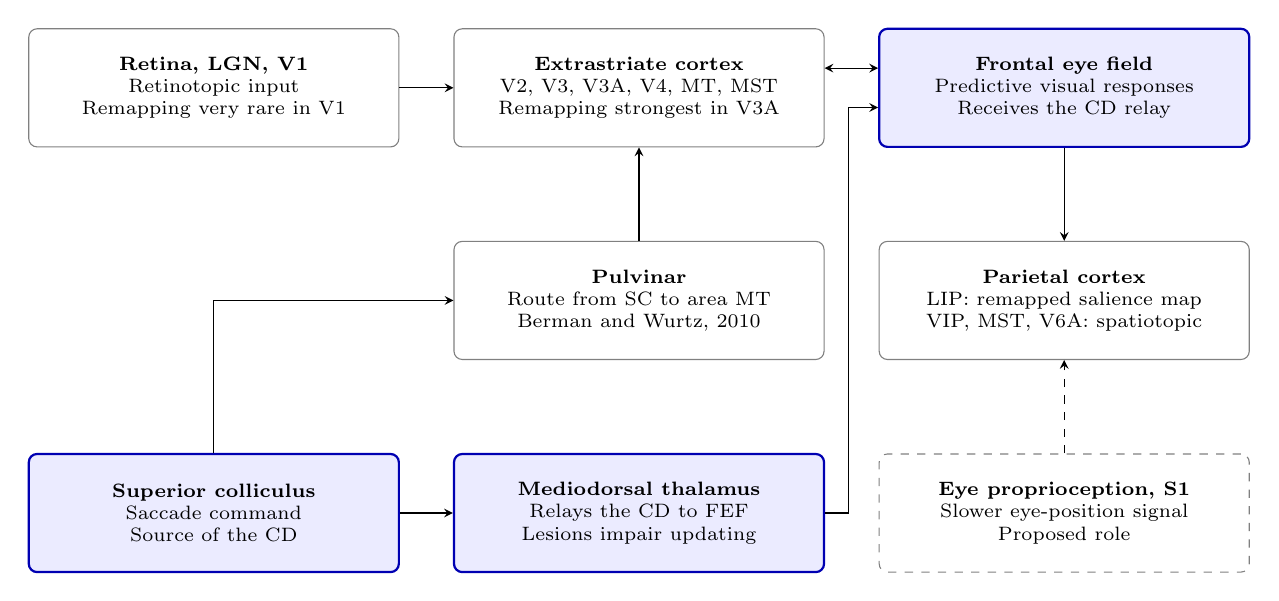
\begin{tikzpicture}[>=stealth,
  box/.style={draw=gray,rounded corners=3pt,minimum width=4.7cm,minimum height=1.5cm,align=center,font=\scriptsize,inner sep=3pt},
  main/.style={box,draw=blue!70!black,fill=blue!8,thick},
  prov/.style={box,dashed}]
\node[box] (retina) at (0,0) {\textbf{Retina, LGN, V1}\\Retinotopic input\\Remapping very rare in V1};
\node[box] (extra) at (5.4,0) {\textbf{Extrastriate cortex}\\V2, V3, V3A, V4, MT, MST\\Remapping strongest in V3A};
\node[main] (fef) at (10.8,0) {\textbf{Frontal eye field}\\Predictive visual responses\\Receives the CD relay};
\node[box] (pulv) at (5.4,-2.7) {\textbf{Pulvinar}\\Route from SC to area MT\\Berman and Wurtz, 2010};
\node[box] (par) at (10.8,-2.7) {\textbf{Parietal cortex}\\LIP: remapped salience map\\VIP, MST, V6A: spatiotopic};
\node[main] (sc) at (0,-5.4) {\textbf{Superior colliculus}\\Saccade command\\Source of the CD};
\node[main] (md) at (5.4,-5.4) {\textbf{Mediodorsal thalamus}\\Relays the CD to FEF\\Lesions impair updating};
\node[prov] (s1) at (10.8,-5.4) {\textbf{Eye proprioception, S1}\\Slower eye-position signal\\Proposed role};
\draw[->] (retina)--(extra);
\draw[<->] ([yshift=0.25cm]extra.east)--([yshift=0.25cm]fef.west);
\draw[->] (sc)--(md);
\draw[->] (md.east)-- ++(0.3,0) |- ([yshift=-0.25cm]fef.west);
\draw[->] (sc.north)|-(pulv.west);
\draw[->] (pulv)--(extra);
\draw[->] (fef)--(par);
\draw[->,dashed] (s1)--(par);
\end{tikzpicture}
\caption{The saccade copy travels from midbrain to cortex through the thalamus. Accent: the monkey route of the corollary discharge (CD). Dashed: proposed, not settled.}
\end{figure}

The accent boxes are the route established by \href{https://doi.org/10.1126/science.1069590}{Sommer and Wurtz (2002)} and \href{https://www.nature.com/articles/nature05279}{(2006)}. Arrows are signal flow as described in the cited papers; the dashed link is a proposal.

{\footnotesize\setlength{\tabcolsep}{3pt}
\begin{longtable}{>{\raggedright\arraybackslash}p{2.94cm}>{\raggedright\arraybackslash}p{4.78cm}>{\raggedright\arraybackslash}p{6.62cm}}
\toprule
\textbf{Region} & \textbf{Hypothesized role} & \textbf{Evidence} \\
\midrule
\endhead
Superior colliculus (SC) & Source of the saccade command and of the CD; some neurons anticipate the visual result of the saccade & Monkey units: \href{https://doi.org/10.1152/jn.1972.35.4.575}{Wurtz and Goldberg, 1972}; \href{https://doi.org/10.1152/jn.1995.73.5.1988}{Walker et al., 1995} \\
\addlinespace[2pt]
Mediodorsal (MD) thalamus & Relay of the CD from SC to FEF; in humans, needed for perceptual stability & Monkey: \href{https://doi.org/10.1126/science.1069590}{Sommer and Wurtz, 2002}, \href{https://www.nature.com/articles/nature05279}{2006}. Human thalamic lesions: \href{https://doi.org/10.1073/pnas.0910742107}{Ostendorf et al., 2010} \\
\addlinespace[2pt]
Pulvinar & Alternative route from SC to area MT & Monkey: \href{https://doi.org/10.1523/JNEUROSCI.6176-09.2010}{Berman and Wurtz, 2010}, \href{https://doi.org/10.1523/JNEUROSCI.4738-10.2011}{2011} \\
\addlinespace[2pt]
Frontal eye field (FEF) & Receives the CD; predictive visual responses and remapping; sends delay and visual signals back to SC & Monkey: \href{https://doi.org/10.1152/jn.1997.78.3.1373}{Umeno and Goldberg, 1997}; \href{https://doi.org/10.1152/jn.2001.85.4.1673}{Sommer and Wurtz, 2001}; \href{https://doi.org/10.1038/nature13149}{Zirnsak et al., 2014}. Human fMRI: \href{https://www.sciencedirect.com/science/article/pii/S1053811916306899}{Fairhall et al., 2017} \\
\addlinespace[2pt]
Lateral intraparietal area (LIP) & Salience map in eye-centred coordinates, updated by the intended saccade & Monkey: \href{https://www.science.org/doi/10.1126/science.1553535}{Duhamel et al., 1992}; \href{https://doi.org/10.1093/cercor/5.5.470}{Colby et al., 1995}; \href{https://www.annualreviews.org/doi/10.1146/annurev.neuro.22.1.319}{Colby and Goldberg, 1999} \\
\addlinespace[2pt]
VIP, MST, V6A & Eye-to-head or world-centred coding in a minority of neurons; MST also remaps a motion memory trace & Monkey: \href{https://www.nature.com/articles/39865}{Duhamel et al., 1997}; \href{https://doi.org/10.1152/jn.1997.77.2.944}{Bremmer et al., 1997}; \href{https://www.sciencedirect.com/science/article/pii/S0896627304003319}{Ilg et al., 2004}; \href{https://doi.org/10.1152/jn.01054.2006}{Inaba et al., 2007}; \href{https://doi.org/10.1073/pnas.1401370111}{Inaba and Kawano, 2014}; V6A: \href{https://doi.org/10.1007/BF00227102}{Galletti et al., 1993} \\
\addlinespace[2pt]
Extrastriate V2, V3, V3A & Remapping, rarer at earlier stages & Monkey: \href{https://doi.org/10.1073/pnas.052379899}{Nakamura and Colby, 2002} \\
\addlinespace[2pt]
V4 & Receptive-field changes around saccades, with more than one type of remapping & Monkey: \href{https://doi.org/10.1016/S0896-6273(01)00250-1}{Tolias et al., 2001}; \href{https://doi.org/10.1038/ncomms10402}{Neupane et al., 2016} \\
\addlinespace[2pt]
V1 & Retinotopic input stage; remapping very rare & Monkey: \href{https://doi.org/10.1073/pnas.052379899}{Nakamura and Colby, 2002} \\
\addlinespace[2pt]
Eye proprioception, primary somatosensory cortex (S1) & Slower eye-position signal, proposed to complement the CD & Monkey: \href{https://doi.org/10.1038/nn1878}{Wang et al., 2007}; review: \href{https://doi.org/10.1146/annurev-vision-082114-035407}{Sun and Goldberg, 2016} \\
\addlinespace[2pt]
Human posterior parietal cortex & Gaze-centred updating of remembered locations; transsaccadic memory; spatiotopic repetition suppression & fMRI: \href{https://doi.org/10.1523/JNEUROSCI.23-15-06209.2003}{Medendorp et al., 2003}; \href{https://doi.org/10.1016/S0896-6273(03)00393-3}{Merriam et al., 2003}; \href{https://www.sciencedirect.com/science/article/pii/S1053811916306899}{Fairhall et al., 2017}. TMS: \href{https://doi.org/10.1523/JNEUROSCI.0542-08.2008}{Prime et al., 2008} \\
\addlinespace[2pt]
Human visual cortex, hMT+ & Spatiotopic selectivity in hMT+, dependent on attention; retinotopic coding in higher visual cortex; remapping in visual areas & fMRI: \href{https://doi.org/10.1038/nn1824}{d'Avossa et al., 2007}; \href{https://doi.org/10.1371/journal.pone.0021661}{Crespi et al., 2011}; \href{https://doi.org/10.1093/cercor/bhr357}{Golomb and Kanwisher, 2012}; \href{https://doi.org/10.1152/jn.00189.2006}{Merriam et al., 2007} \\
\addlinespace[2pt]
\bottomrule
\end{longtable}}

\section{The story in publications}

The field moves from signal (CD) to neurons (remapping, gain fields) to a human reference-frame contest, then to timing; ``In library'' marks papers in the Zotero collection.

{\footnotesize\setlength{\tabcolsep}{3pt}
\begin{longtable}{>{\raggedright\arraybackslash}p{0.83cm}>{\raggedright\arraybackslash}p{3.31cm}>{\raggedright\arraybackslash}p{1.75cm}>{\raggedright\arraybackslash}p{3.77cm}>{\raggedright\arraybackslash}p{3.68cm}>{\raggedright\arraybackslash}p{1.10cm}}
\toprule
\textbf{Year} & \textbf{Paper} & \textbf{Line} & \textbf{Paradigm} & \textbf{Finding} & \textbf{In lib.} \\
\midrule
\endhead
1983 & Andersen and Mountcastle & Spatiotopic & Monkey parietal single units, eye-position gain & Eye position multiplicatively scales visual responses (gain fields) & No \\
\addlinespace[2pt]
1983 & \href{https://www.jstor.org/stable/1690996}{Guthrie, Porter, Sparks} & CD & Collicular microstimulation perturbs a saccade, proprioception eliminated & Eye-position information is internal, not reafferent & Yes \\
\addlinespace[2pt]
1992 & \href{https://www.science.org/doi/10.1126/science.1553535}{Duhamel, Colby, Goldberg} & Retinotopic & Monkey LIP single units, double-step saccade task & Predictive receptive-field remapping before the saccade & Yes \\
\addlinespace[2pt]
1997 & \href{https://www.nature.com/articles/39865}{Duhamel, Bremmer, BenHamed, Graf} & Spatiotopic & Monkey VIP units, fixation at several gaze angles & Receptive fields on an eye-to-head continuum & Yes \\
\addlinespace[2pt]
1999 & \href{https://www.annualreviews.org/doi/10.1146/annurev.neuro.22.1.319}{Colby, Goldberg} & Retinotopic & Review of parietal physiology & LIP salience map updated by intended movement & Yes \\
\addlinespace[2pt]
2002 & Nakamura, Colby & Retinotopic & Monkey V3A, V3, V2, V1 units, stimulus flashed in old or new RF around a saccade & Remapping reaches early visual cortex & No \\
\addlinespace[2pt]
2004 & \href{https://www.sciencedirect.com/science/article/pii/S0896627304003319}{Ilg, Schumann, Thier} & Spatiotopic & Monkey MST units during pursuit & World-centred target-motion signals & Yes \\
\addlinespace[2pt]
2005 & Melcher & Spatiotopic & Human psychophysics, form adaptation across a saccade & Form aftereffects transfer to the same spatial position; transfer grows with stimulus complexity & No \\
\addlinespace[2pt]
2006 & Sommer, Wurtz & CD & Monkey FEF units, thalamic inactivation & A collicular, thalamic CD pathway drives remapping & No \\
\addlinespace[2pt]
2008 & Wurtz & CD, Retinotopic & Review & Remapping plus suppression as stability mechanisms & No \\
\addlinespace[2pt]
2010 & Cavanagh, Hunt, Afraz, Rolfs & Retinotopic & Theory with psychophysics & Remapped attention pointers, not a map & No \\
\addlinespace[2pt]
2011 & Rolfs, Jonikaitis, Deubel, Cavanagh & Retinotopic & Human attention probe before a saccade & Attention shifts to the post-saccadic location predictively & No \\
\addlinespace[2pt]
2012 & \href{https://royalsocietypublishing.org/doi/10.1098/rspb.2012.0637}{Turi, Burr} & Spatiotopic & Human psychophysics, positional motion aftereffect & Spatiotopic position map, retinotopic classic aftereffect & Yes \\
\addlinespace[2pt]
2012 & Golomb, Kanwisher & Retinotopic & Human fMRI MVPA, saccade between locations & Higher cortex codes location retinotopically & No \\
\addlinespace[2pt]
2013 & Zimmermann, Morrone, Fink, Burr & Spatiotopic & Human psychophysics, build-up of spatiotopic effects over time & Spatiotopic maps build over hundreds of ms & No \\
\addlinespace[2pt]
2014 & Zirnsak, Steinmetz, Noudoost, Moore & Retinotopic & Monkey FEF units, mapped RFs across the saccade & Receptive fields converge on the saccade target & No \\
\addlinespace[2pt]
2017 & \href{https://www.sciencedirect.com/science/article/pii/S1053811916306899}{Fairhall et al.} & Spatiotopic & Human fMRI repetition suppression across a saccade & Spatiotopic suppression in parietal cortex, FEF & Yes \\
\addlinespace[2pt]
2018 & \href{https://www.annualreviews.org/content/journals/10.1146/annurev-vision-091517-034317}{Binda, Morrone} & Both & Review of perisaccadic psychophysics & CD links suppression, compression and remapping & Yes \\
\addlinespace[2pt]
2019 & \href{https://www.pnas.org/doi/10.1073/pnas.1812210116}{Fabius et al.} & Spatiotopic & Human gaze-contingent high-phi & Spatiotopic updating within 150 ms & Yes \\
\addlinespace[2pt]
\bottomrule
\end{longtable}}

Paradigm families, in order of what they isolate: single-unit receptive-field mapping around saccades (remapping), reference-frame competition in adaptation and fMRI (the spatiotopic versus retinotopic contest), and gaze-contingent apparent-motion probes (timing).

\section{Synthesis and open questions}

The two lines now look complementary more than rival: fast, predictive, retinotopic remapping covers the saccade itself, and a slower, sparser spatiotopic signal builds afterwards.

\begin{itemize}[itemsep=2pt,topsep=2pt]
\item \textbf{Timing reconciles them.} Remapping acts before and at the saccade. Spatiotopic effects were measured as slow (Zimmermann et al., 2013) until a continuous gaze-contingent probe found them within 150 ms (Fabius et al., 2019). The paradigm, not only the brain, set the estimate.
\item \textbf{Spatiotopy may be partial.} Only a minority of neurons are spatiotopic, and Golomb and Kanwisher (2012) find retinotopic coding even in higher cortex, while Fairhall et al. (2017) find spatiotopic repetition suppression in parietal cortex and FEF. Task and stimulus choice (position adaptation vs object identity) seem to decide which frame wins.
\item \textbf{Deflationary alternative.} O'Regan and Noe (2001) and Irwin (1991) argue that trans-saccadic memory is small and the scene is re-sampled, so stability needs no map. Cavanagh et al.'s attention pointers are a middle way: a few tracked locations.
\item \textbf{Open.} Whether remapping carries feature content or only location, how the world-centred signal is read out, and how voluntary and reflexive saccades differ.
\end{itemize}

\textbf{For the Kanizsa saliences model.} A voluntary-saccade model faces the same choice: keep representations retinotopic and shift them with the planned saccade (line B), or maintain a world-centred salience map (line A). The project's own finding that the saccade reset mask is nearly flat, so salience saccades undo goal saccades, is the model-side analogue of a remapping signal that does not carry what was already attended; a CD-style, saccade-aware shift is the biologically motivated fix, with a slower spatiotopic store as a second option.

\section*{References}
\addcontentsline{toc}{section}{References}

Library papers were read (abstracts and introductions) in the Zotero folder \texttt{Elementi visual\_stability}; every other reference was checked on 2026-10-04 against Crossref or Europe PMC for authors, year, venue and DOI. Publisher links return 403 to scripts, so they were checked through their DOIs, not by opening the page.

\textbf{In the library (9)}

\begin{itemize}[itemsep=2pt,topsep=2pt]
\item Binda, P., and Morrone, M. C. (2018). Vision during saccadic eye movements. Annu Rev Vis Sci. \href{https://doi.org/10.1146/annurev-vision-091517-034317}{doi:10.1146/annurev-vision-091517-034317}
\item Colby, C. L., and Goldberg, M. E. (1999). Space and attention in parietal cortex. Annu Rev Neurosci 22. \href{https://doi.org/10.1146/annurev.neuro.22.1.319}{doi:10.1146/annurev.neuro.22.1.319}
\item Duhamel, J.-R., Bremmer, F., BenHamed, S., and Graf, W. (1997). Spatial invariance of visual receptive fields in parietal cortex neurons. Nature 389. \href{https://doi.org/10.1038/39865}{doi:10.1038/39865}
\item Duhamel, J.-R., Colby, C. L., and Goldberg, M. E. (1992). The updating of the representation of visual space in parietal cortex by intended eye movements. Science 255, 90-92. \href{https://doi.org/10.1126/science.1553535}{doi:10.1126/science.1553535}
\item Fabius, J. H., Fracasso, A., Nijboer, T. C. W., and Van der Stigchel, S. (2019). Time course of spatiotopic updating across saccades. PNAS 116. \href{https://doi.org/10.1073/pnas.1812210116}{doi:10.1073/pnas.1812210116}
\item Fairhall, S. L., Schwarzbach, J., Lingnau, A., Van Koningsbruggen, M. G., and Melcher, D. (2017). Spatiotopic updating across saccades revealed by spatially-specific fMRI adaptation. NeuroImage 147. \href{https://doi.org/10.1016/j.neuroimage.2016.11.071}{doi:10.1016/j.neuroimage.2016.11.071}
\item Guthrie, B. L., Porter, J. D., and Sparks, D. L. (1983). Corollary discharge provides accurate eye position information to the oculomotor system. Science 221, 1193-1195. \href{https://doi.org/10.1126/science.6612334}{doi:10.1126/science.6612334}
\item Ilg, U. J., Schumann, S., and Thier, P. (2004). Posterior parietal cortex neurons encode target motion in world-centered coordinates. Neuron 43, 145-151. \href{https://doi.org/10.1016/j.neuron.2004.06.006}{doi:10.1016/j.neuron.2004.06.006}
\item Turi, M., and Burr, D. (2012). Spatiotopic perceptual maps in humans: evidence from motion adaptation. Proc R Soc B 279, 3091-3097. \href{https://doi.org/10.1098/rspb.2012.0637}{doi:10.1098/rspb.2012.0637}
\end{itemize}

\textbf{Added }\textbf{references, recent}

\begin{itemize}[itemsep=2pt,topsep=2pt]
\item Cavanagh, P., Hunt, A. R., Afraz, A., and Rolfs, M. (2010). Visual stability based on remapping of attention pointers. Trends Cogn Sci 14, 147-153. \href{https://doi.org/10.1016/j.tics.2010.01.007}{doi:10.1016/j.tics.2010.01.007}
\item Golomb, J. D., and Kanwisher, N. (2012). Higher level visual cortex represents retinotopic, not spatiotopic, object location. Cereb Cortex 22, 2794-2810. \href{https://doi.org/10.1093/cercor/bhr357}{doi:10.1093/cercor/bhr357}
\item Golomb, J. D., and Kanwisher, N. (2012). Retinotopic memory is more precise than spatiotopic memory. PNAS 109, 1796-1801. \href{https://doi.org/10.1073/pnas.1113168109}{doi:10.1073/pnas.1113168109}
\item Sommer, M. A., and Wurtz, R. H. (2006). Influence of the thalamus on spatial visual processing in frontal cortex. Nature 444, 374-377. \href{https://doi.org/10.1038/nature05279}{doi:10.1038/nature05279}
\item Wurtz, R. H. (2008). Neuronal mechanisms of visual stability. Vision Res 48, 2070-2089. \href{https://doi.org/10.1016/j.visres.2008.03.021}{doi:10.1016/j.visres.2008.03.021} \href{https://pubmed.ncbi.nlm.nih.gov/18513781/}{PubMed}
\item Zimmermann, E., Morrone, M. C., Fink, G. R., and Burr, D. (2013). Spatiotopic neural representations develop slowly across saccades. Curr Biol 23, R193-R194. \href{https://doi.org/10.1016/j.cub.2013.01.065}{doi:10.1016/j.cub.2013.01.065} \href{https://pubmed.ncbi.nlm.nih.gov/23473558/}{PubMed}
\end{itemize}

\textbf{Added }\textbf{references, earlier and background}

\begin{itemize}[itemsep=2pt,topsep=2pt]
\item Andersen, R. A., and Mountcastle, V. B. (1983). The influence of the angle of gaze upon the excitability of the light-sensitive neurons of the posterior parietal cortex. J Neurosci 3, 532-548. \href{https://doi.org/10.1523/JNEUROSCI.03-03-00532.1983}{doi:10.1523/JNEUROSCI.03-03-00532.1983}
\item Irwin, D. E. (1991). Information integration across saccadic eye movements. Cogn Psychol 23, 420-456. \href{https://doi.org/10.1016/0010-0285(91)90015-G}{doi:10.1016/0010-0285(91)90015-G}
\item Melcher, D. (2005). Spatiotopic transfer of visual-form adaptation across saccadic eye movements. Curr Biol 15, 1745-1748. \href{https://doi.org/10.1016/j.cub.2005.08.044}{doi:10.1016/j.cub.2005.08.044}
\item Nakamura, K., and Colby, C. L. (2002). Updating of the visual representation in monkey striate and extrastriate cortex during saccades. PNAS 99, 4026-4031. \href{https://doi.org/10.1073/pnas.052379899}{doi:10.1073/pnas.052379899}
\item O'Regan, J. K., and Noe, A. (2001). A sensorimotor account of vision and visual consciousness. Behav Brain Sci 24, 939-973. \href{https://doi.org/10.1017/S0140525X01000115}{doi:10.1017/S0140525X01000115}
\item Rolfs, M., Jonikaitis, D., Deubel, H., and Cavanagh, P. (2011). Predictive remapping of attention across eye movements. Nat Neurosci 14, 252-256. \href{https://doi.org/10.1038/nn.2711}{doi:10.1038/nn.2711}
\item Sperry, R. W. (1950). Neural basis of the spontaneous optokinetic response produced by visual inversion. J Comp Physiol Psychol 43, 482-489. \href{https://doi.org/10.1037/h0055479}{doi:10.1037/h0055479}
\item von Holst, E., and Mittelstaedt, H. (1950). Das Reafferenzprinzip. Naturwissenschaften 37, 464-476. \href{https://doi.org/10.1007/BF00622503}{doi:10.1007/BF00622503}
\item Zirnsak, M., Steinmetz, N. A., Noudoost, B., Xu, K. Z., and Moore, T. (2014). Visual space is compressed in prefrontal cortex before eye movements. Nature 507, 504-507. \href{https://doi.org/10.1038/nature13149}{doi:10.1038/nature13149}
\end{itemize}

\begin{itemize}[itemsep=2pt,topsep=2pt]
\item Bridgeman, B., Hendry, D., and Stark, L. (1975). Failure to detect displacement of the visual world during saccadic eye movements. Vision Res 15, 719-722. \href{https://doi.org/10.1016/0042-6989(75)90290-4}{doi:10.1016/0042-6989(75)90290-4}
\item Burr, D. C., and Morrone, M. C. (2011). Spatiotopic coding and remapping in humans. Phil Trans R Soc B 366, 504-515. \href{https://doi.org/10.1098/rstb.2010.0244}{doi:10.1098/rstb.2010.0244}
\item Crapse, T. B., and Sommer, M. A. (2008). Corollary discharge across the animal kingdom. Nat Rev Neurosci 9, 587-600. \href{https://doi.org/10.1038/nrn2457}{doi:10.1038/nrn2457}
\item Deubel, H., Schneider, W. X., and Bridgeman, B. (1996). Postsaccadic target blanking prevents saccadic suppression of image displacement. Vision Res 36, 985-996. \href{https://doi.org/10.1016/0042-6989(95)00203-0}{doi:10.1016/0042-6989(95)00203-0}
\item Morris, A. P., Kubischik, M., Hoffmann, K.-P., Krekelberg, B., and Bremmer, F. (2012). Dynamics of eye-position signals in the dorsal visual system. Curr Biol 22, 173-179. \href{https://doi.org/10.1016/j.cub.2011.12.032}{doi:10.1016/j.cub.2011.12.032}
\item Niemeier, M., Crawford, J. D., and Tweed, D. B. (2003). Optimal transsaccadic integration explains distorted spatial perception. Nature 422, 76-80. \href{https://doi.org/10.1038/nature01439}{doi:10.1038/nature01439}
\item Rao, H. M., Mayo, J. P., and Sommer, M. A. (2016). Circuits for presaccadic visual remapping. J Neurophysiol 116, 2624-2636. \href{https://doi.org/10.1152/jn.00182.2016}{doi:10.1152/jn.00182.2016}
\item Ross, J., Morrone, M. C., Goldberg, M. E., and Burr, D. C. (2001). Changes in visual perception at the time of saccades. Trends Neurosci 24, 113-121. \href{https://doi.org/10.1016/S0166-2236(00)01685-4}{doi:10.1016/S0166-2236(00)01685-4}
\item Sommer, M. A., and Wurtz, R. H. (2002). A pathway in primate brain for internal monitoring of movements. Science 296, 1480-1482. \href{https://doi.org/10.1126/science.1069590}{doi:10.1126/science.1069590}
\item Sommer, M. A., and Wurtz, R. H. (2008). Brain circuits for the internal monitoring of movements. Annu Rev Neurosci 31, 317-338. \href{https://doi.org/10.1146/annurev.neuro.31.060407.125627}{doi:10.1146/annurev.neuro.31.060407.125627}
\item Sun, L. D., and Goldberg, M. E. (2016). Corollary discharge and oculomotor proprioception: cortical mechanisms for spatially accurate vision. Annu Rev Vis Sci 2, 61-84. \href{https://doi.org/10.1146/annurev-vision-082114-035407}{doi:10.1146/annurev-vision-082114-035407}
\item Wang, X., Zhang, M., Cohen, I. S., and Goldberg, M. E. (2007). The proprioceptive representation of eye position in monkey primary somatosensory cortex. Nat Neurosci 10, 640-646. \href{https://doi.org/10.1038/nn1878}{doi:10.1038/nn1878}
\item Xu, B. Y., Karachi, C., and Goldberg, M. E. (2012). The postsaccadic unreliability of gain fields renders it unlikely that the motor system can use them to calculate target position in space. Neuron 76, 1201-1209. \href{https://doi.org/10.1016/j.neuron.2012.10.034}{doi:10.1016/j.neuron.2012.10.034}
\end{itemize}

\begin{itemize}[itemsep=2pt,topsep=2pt]
\item Berman, R. A., and Wurtz, R. H. (2010). Functional identification of a pulvinar path from superior colliculus to cortical area MT. J Neurosci 30, 6342-6354. \href{https://doi.org/10.1523/JNEUROSCI.6176-09.2010}{doi:10.1523/JNEUROSCI.6176-09.2010}
\item Berman, R. A., and Wurtz, R. H. (2011). Signals conveyed in the pulvinar pathway from superior colliculus to cortical area MT. J Neurosci 31, 373-384. \href{https://doi.org/10.1523/JNEUROSCI.4738-10.2011}{doi:10.1523/JNEUROSCI.4738-10.2011}
\item Bremmer, F., Ilg, U. J., Thiele, A., Distler, C., and Hoffmann, K.-P. (1997). Eye position effects in monkey cortex. I. Visual and pursuit-related activity in extrastriate areas MT and MST. J Neurophysiol 77, 944-961. \href{https://doi.org/10.1152/jn.1997.77.2.944}{doi:10.1152/jn.1997.77.2.944}
\item Colby, C. L., Duhamel, J.-R., and Goldberg, M. E. (1995). Oculocentric spatial representation in parietal cortex. Cereb Cortex 5, 470-481. \href{https://doi.org/10.1093/cercor/5.5.470}{doi:10.1093/cercor/5.5.470}
\item Crespi, S., Biagi, L., d'Avossa, G., Burr, D. C., Tosetti, M., and Morrone, M. C. (2011). Spatiotopic coding of BOLD signal in human visual cortex depends on spatial attention. PLoS ONE 6, e21661. \href{https://doi.org/10.1371/journal.pone.0021661}{doi:10.1371/journal.pone.0021661}
\item d'Avossa, G., Tosetti, M., Crespi, S., Biagi, L., Burr, D. C., and Morrone, M. C. (2007). Spatiotopic selectivity of BOLD responses to visual motion in human area MT. Nat Neurosci 10, 249-255. \href{https://doi.org/10.1038/nn1824}{doi:10.1038/nn1824}
\item Galletti, C., Battaglini, P. P., and Fattori, P. (1993). Parietal neurons encoding spatial locations in craniotopic coordinates. Exp Brain Res 96. \href{https://doi.org/10.1007/BF00227102}{doi:10.1007/BF00227102}
\item Inaba, N., and Kawano, K. (2014). Neurons in cortical area MST remap the memory trace of visual motion across saccadic eye movements. PNAS 111, 7825-7830. \href{https://doi.org/10.1073/pnas.1401370111}{doi:10.1073/pnas.1401370111}
\item Inaba, N., Shinomoto, S., Yamane, S., Takemura, A., and Kawano, K. (2007). MST neurons code for visual motion in space independent of pursuit eye movements. J Neurophysiol 97, 3473-3483. \href{https://doi.org/10.1152/jn.01054.2006}{doi:10.1152/jn.01054.2006}
\item Medendorp, W. P., Goltz, H. C., Vilis, T., and Crawford, J. D. (2003). Gaze-centered updating of visual space in human parietal cortex. J Neurosci 23, 6209-6214. \href{https://doi.org/10.1523/JNEUROSCI.23-15-06209.2003}{doi:10.1523/JNEUROSCI.23-15-06209.2003}
\item Merriam, E. P., Genovese, C. R., and Colby, C. L. (2003). Spatial updating in human parietal cortex. Neuron 39, 361-373. \href{https://doi.org/10.1016/S0896-6273(03)00393-3}{doi:10.1016/S0896-6273(03)00393-3}
\item Merriam, E. P., Genovese, C. R., and Colby, C. L. (2007). Remapping in human visual cortex. J Neurophysiol 97, 1738-1755. \href{https://doi.org/10.1152/jn.00189.2006}{doi:10.1152/jn.00189.2006}
\item Neupane, S., Guitton, D., and Pack, C. C. (2016). Two distinct types of remapping in primate cortical area V4. Nat Commun 7, 10402. \href{https://doi.org/10.1038/ncomms10402}{doi:10.1038/ncomms10402}
\item Ostendorf, F., Liebermann, D., and Ploner, C. J. (2010). Human thalamus contributes to perceptual stability across eye movements. PNAS 107, 1229-1234. \href{https://doi.org/10.1073/pnas.0910742107}{doi:10.1073/pnas.0910742107}
\item Prime, S. L., Vesia, M., and Crawford, J. D. (2008). Transcranial magnetic stimulation over posterior parietal cortex disrupts transsaccadic memory of multiple objects. J Neurosci 28, 6938-6949. \href{https://doi.org/10.1523/JNEUROSCI.0542-08.2008}{doi:10.1523/JNEUROSCI.0542-08.2008}
\item Sommer, M. A., and Wurtz, R. H. (2001). Frontal eye field sends delay activity related to movement, memory, and vision to the superior colliculus. J Neurophysiol 85, 1673-1685. \href{https://doi.org/10.1152/jn.2001.85.4.1673}{doi:10.1152/jn.2001.85.4.1673}
\item Tolias, A. S., Moore, T., Smirnakis, S. M., Tehovnik, E. J., Siapas, A. G., and Schiller, P. H. (2001). Eye movements modulate visual receptive fields of V4 neurons. Neuron 29, 757-767. \href{https://doi.org/10.1016/S0896-6273(01)00250-1}{doi:10.1016/S0896-6273(01)00250-1}
\item Umeno, M. M., and Goldberg, M. E. (1997). Spatial processing in the monkey frontal eye field. I. Predictive visual responses. J Neurophysiol 78, 1373-1383. \href{https://doi.org/10.1152/jn.1997.78.3.1373}{doi:10.1152/jn.1997.78.3.1373}
\item Walker, M. F., Fitzgibbon, E. J., and Goldberg, M. E. (1995). Neurons in the monkey superior colliculus predict the visual result of impending saccadic eye movements. J Neurophysiol 73, 1988-2003. \href{https://doi.org/10.1152/jn.1995.73.5.1988}{doi:10.1152/jn.1995.73.5.1988}
\item Wurtz, R. H., and Goldberg, M. E. (1972). Activity of superior colliculus in behaving monkey. III. Cells discharging before eye movements. J Neurophysiol 35, 575-586. \href{https://doi.org/10.1152/jn.1972.35.4.575}{doi:10.1152/jn.1972.35.4.575}
\end{itemize}

\end{document}
